%
% Unless otherwise indicated, the copyright in this material is 
% owned by Joerg Evermann. This material is licensed to you under the 
% Creative Commons by-attribution non-commercial license (CC BY-NC 4.0)}
%


\section{Introduction}

This section describes some of the terminology around the rapidly expanding field of data analytics, business analytics, data science, statistics, machine learning and AI (artificial intelligence). 

\emph{Data analytics} (or simply 'analytics') refers to the broad collection of methods, techniques, and tools to allow humans to make sense of information for purposes of understanding and decision making. Business analytics is the application of data analytics to operational, tactical, or strategic management in businesses and other organizations. Examples are the use of visualization of human resource performance data, trend analysis of outbound logistics costs, prediction of customer demand, fraud analysis of financial transactions, and others.

Data analytics as a broad field is closely related to a range of other fields, such as data management (how best to collect, store, access, and use data in a variety of format), visualization (how best to present data in an easy-to-understand format to generate insights or persuade stakeholders), machine learning (how to train computers to classify data and to make predictions), or text analysis (how to extract meaningful information from natural-language text information). Some argue that these fields are within analytics, but others view them as separate but strongly interrelated. For example, text analysis and machine learning overlap when training computers to predict customer behaviour based on social media post data. Text analysis can provide certain features that characterize or summarize a text, and may be used as input for machine learning. Machine learning models can exploit text-specific features, such as the sentence structure, in making predictions. Training machine learning systems also requires a very large amount of data, so advanced data management techniques are required in order to store and provide this data in an efficient way. 

\emph{Artificial Intelligence (AI)} is a field with a long and varied history, going back to the 1960s. Originally, AI was used for symbolic computations, where researchers attempted to explicitly describe and model human reasoning processes in a computer. In the late 1990s and early 2000s, AI has morphed to focus on statistical models and has most recently become dominated by artificial neural networks (ANN) and deep neural networks (DNN), a field called deep learning. Artificial neural networks, while inspired by the human brain, are essentially statistical models for classification and regression, akin to the simple linear or logistic regression. But whereas the simplest linear regression model may describe a small dataset of hundreds to thousands of observations using just two parameters (the slope and intercept), ANN and DNN are non-linear and highly complex with millions or even billions of parameters and are often trained on billions of observations. However, the main ideas are the same in that the model is trained on or fitted to a data set. 

More recently, since about 2020, \emph{generative AI}, that is, AI models and systems that are used to generate text, images, audio or video in response to user input has become synonymous with AI. The rise in popularity of systems such as ChatGPT, Dall-E, and many others, has led to many people equating AI with generative AI.

While \emph{machine learning} may sometimes be viewed synonymously with ANN or DNN, the field of machine learning is broader than just neural network models and concerns the development of methods to make predictions for new observations. Traditional statistical techniques for regression and classification, such as decision trees or support vector machines, are considered part of machine learning, and therefore also part of data analytics. However, these statistical models sometimes take a back seat role compared to ANNs because of the power and flexibility of the latter. 

Machine learning and AI are also sometimes viewed synonymously. However, as noted above, there are subfields of AI that are not concerned with machine learning and prediction. First, research into symbolic reasoning is still ongoing. Second, methods such as reinforcement learning, which focuses not on making predictions, but on prescribing optimal courses of action, are considered part of machine learning and AI.

\emph{Big Data} was an important topic in the early 2000s and 2010s but is now often considered a sub-field of data analytics or data science. The motivation for Big Data was the recognition that the volume of data produced and available for analysis has been growing exponentially since the 1990s. This has spurred the development of advanced data management methods, techniques, and tools, such as distributed file systems and databases. The velocity of data, that is, its rate of production, has also increased greatly since the 1990s. Processing the data often has to occur in real-time, leading to development of techniques and tools that can analyze data ''on-the-fly'' (''stream processing'').

Finally, the term \emph{data science} is often used in a less applied and more scientific or research and developmental way than the term data analytics, to characterize the development, rather than application, of methods, techniques, and tools.

\section{Methods, Techniques, and Tools}

In the context of data science and data analytics, methods, techniques, and tools play distinct roles in the process of extracting insights from data. \emph{Methods} encompass overarching approaches and strategies, providing a systematic framework for tasks such as data exploration, modeling, and analysis. These high-level methodologies guide data scientists in formulating a structured plan for addressing specific challenges or achieving analytical goals.

\emph{Techniques} in data science are the specific procedures and practices employed within the broader methodological framework. These practical and detailed approaches are applied to handle particular aspects of the data analysis process. For instance, in exploratory data analysis, techniques like histograms or scatter plots are used to visually inspect data distributions or relationships between variables and in classification, a naive Bayes classifier is considered a specific technique.

\emph{Tools} in data science refer to the instruments and software applications that facilitate the practical application of methods and techniques. These can range from programming languages like Python and R, statistical packages such as Pandas and SciPy, to visualization tools like Shiny or Matplotlib. The selection of appropriate tools is crucial for efficiently executing data science tasks and optimizing the workflow.

\section{Types of Analytics}

There are different ''types'' of analytics that have different aims. 

\paragraph*{Descriptive Analytics} describes ''what is''. It typically provides summaries of the data, makes comparisons between different types of entities or measurements, may identify historical trends, or provide rankings of observations or measurements. An example is the identification and comparison of current and historical costs to manufacture different widgets in different plants. Another example are the identification of the top-grossing sales people in the organization for specific product types, or calculating the the mean cycle time of the order-to-cash business process for different time periods. Descriptive analytics is therefore important in a business context and organizations expend a great deal of money, time, and effort on technologies such as report generating tools to support this type of analytics. 

\paragraph*{Predictive Analytics} describes ''what may be'' in the future. It typically builds a \emph{model} based on past data to predict future cases/events/outcomes. As a simple example, consider a linear regression model that predicts the overall spending of a customer from their income. One can build a linear model with parameters for the intercept and slope and then train the model on customers whose spending and income are known. Training means to determine the two parameters of the model so that they model best fits the data. Given a trained model, one can then predict the overall spending of a new customer given their income. Of course, the models can be much more complex than a simple linear regression, and often have tens, hundreds, thousands, or even millions of parameters, but the principle of model-based predictive analytics remains the same.

\paragraph*{Prescriptive Analytics} describes ''what should be done''. Similar to predictive analytics, a model is usually built from  past data. However, the model must now also consider which actions can be taken (and were taken for the past training data). In reinforcement learning, a popular prescriptive analytics technique, one assumes that an \emph{agent} can observe the state of an \emph{environment}, can take \emph{actions} based on the observed state, and receives a (positive or negative) reward from the environment after taking an action. Actions may change the state of the environment. The agent must learn to identify those actions in each state that give it the maximum rewards. The optimal actions are called a \emph{policy} and can then be used to prescribe which action to take in which state.

\paragraph*{Visual Analytics} describes the use of graphs (plots, diagrams) to visualize information for exploring data and gaining insight. Visual analytics makes use of the human ability to visually identify trends, make comparisons, etc. In effect, this type of analytics supports humans in their tasks. It employs no mathematical or statistical models. However, humans may identify features of the data such as trends, comparisons, etc. with visual analytics that may then be tested with statistical models or form the basis on which to build predictive or prescriptive analytics models. 

\section{Machine Learning}

In the context of analytics, machine learning (sometimes simply called ''learning'') can be divided into supervised and unsupervised learning. \emph{Supervised learning} is typically based on a parameterized statistical or mathematical model. For example, a simple linear regression is based on two parameters, the slope and intercept. Models are trained (that is, parameters are estimated) by adjusting the model parameters so that the model's output (e.g. the predicts value ''$\hat{y}$ in a linear regression) for each given input (e.g. the ''x'' value in a linear regression) matches the actually observed outcome (the ''y'' value in a linear regression). Supervised learning assumes that a correct/observed outcome is available for all inputs. Linear regression is a very simple supervised learning approach with a simple statistical model; on the other extreme there are generative pre-trained transformer (GPT) models that predict words for generating text, and which contain billions of parameters and non-linear relationships among them.

\emph{Unsupervised learning} on the other hand does not require outcome values and only requires ''input'' (''x'') values. Typical unsupervised learning tasks are clustering and dimensionality reduction. For example, one may form clusters of widgets at the end of a production line based on how similar the widgets are on different characteristics that were measured by sensors. These clusters could then, for example, be interpreted as quality grades. Similarly, customers may be clustered based on their past transactions or purchases. Different marketing strategies may then be applied to each cluster. The aim of dimensionality reduction is to be able to describe a data set with many variables by using only a few variables. Imagine that having hundreds of different characteristics of widgets. One might then wish to simplify and identify fewer, perhaps as few as two or three, combinations of the original characteristics that provide the same information about the widgets.

\section{Analytics is not Statistics}

Analytics and statistics use the same kinds of mathematical models. However, ''traditional'' \emph{statistics} focuses on sample and population characteristics, such asmeans, slopes, intercepts, and others, of a sample or a population that are represented as parameters of a mathematical model. Statistics aims to identify and explain the data generating mechanism, i.e. the ''real world'' or population. In particular, \emph{inferential statistics} is used to generalize from a sample to a population. Importantly, statistics is typically not concerned with individual cases or individual observations.

In contrast, data analytics, especially predictive analytics, focuses on predicting the outcome of an individual case or observation. Analytics is pragmatic, in that models are considered useful tools and do not need to faithfully describe the ''real world'' or the data generating mechanism, as long as they make good predictions or are otherwise useful for their purpose. Consequently, there is no inference from sample to population, because the model does not claim to describe a population. The quality of a model is determined not by its fit with the observed data, but by its precision or accuracy when predicting specific observations. 

\section{Tools used in this Course}

The software used in this course is open-source and free software. Open-source software (OSS) embodies a collaborative approach to software development, allowing users to access, modify, and distribute the source code freely\footnote{\url{https://en.wikipedia.org/wiki/Open-source_software}}. This approach promotes transparency, enabling users to inspect the code, modify, adapt, fix and extend it, and contribute to its improvement. 

Free software, as defined by the Free Software Foundation (FSF), goes beyond accessibility, emphasizing users' fundamental freedoms to run, study, modify, and share the software\footnote{\url{https://en.wikipedia.org/wiki/Free_software}}. Contrary to the common misconception, "free" in this context pertains to freedom, not necessarily zero cost. The ethical philosophy behind free software underscores the importance of user control over technology. 

The term FOSS, or Free and Open-Source Software\footnote{\url{https://en.wikipedia.org/wiki/Free_and_open-source_software}}, serves as an inclusive label encompassing both the principles of free software and the collaborative nature of open-source software. FOSS encourages a shared approach to software development, emphasizing not only the technical benefits of open code but also the ethical imperative of user freedom and community-driven innovation.

Free and Open-Source Software (FOSS) \emph{licenses} are legal agreements that govern the use, modification, and distribution of open-source software. These licenses play a crucial role in preserving the core principles of freedom, transparency, and collaboration within the open-source community. Common characteristics of FOSS licenses are:

\paragraph*{Freedom to Use} FOSS licenses grant users the freedom to use the software for any purpose without any restrictions.

\paragraph*{Freedom to Study} Users have the right to access and study the source code of the software. This transparency allows for a deeper understanding of how the software functions.

\paragraph*{Freedom to Modify} FOSS licenses typically allow users to modify the source code according to their needs. This encourages innovation, customization, and adaptation of the software.

\paragraph*{Freedom to Share} Users can distribute both the original and modified versions of the software, fostering a collaborative environment. This freedom to share is fundamental to the open-source philosophy.

\paragraph*{Copyleft Licenses} Some FOSS licenses, such as the GNU General Public License (GPL), include copyleft provisions. Copyleft ensures that any derivative works or modifications are also subject to the same open-source terms. This prevents the software from being incorporated into proprietary projects without maintaining open-source characteristics.

\paragraph*{Permissive Licenses} On the other hand, permissive licenses, like the MIT License and the Apache License, allow for more flexibility. They permit the use of the software in proprietary projects without imposing the requirement to open-source the derived code.

While a lot of free and open-source software used to be developed by individuals, increasingly FOSS is developed by companies whose business model rests either on providing paid support for such tools, or on providing paid hosted versions of the software, or on providing non-free extensions for their FOSS software. In other cases, companies provide software developer time to important projects that benefit themselves.

\begin{table}
\small
\centering

\begin{tabular}{l|l|l} \hline
R & 4.1.2 & \url{www.r-project.org}\\ 
dplyr & 1.1.3 & \url{www.tidyverse.org} \\
tidyr & 1.3.0 & \url{www.tidyverse.org} \\
ggplot2 & 3.4.4 & \url{www.tidyverse.org} \\
Python & 3.8 & \url{www.python.org} \\
numpy & 1.24.4 & \url{numpy.org} \\
pandas & 2.0.3 & \url{pandas.pydata.org} \\
plotly & 5.18.0 & \url{plotly.com} \\ 
tensorflow & 2.13.1 & \url{www.tensorflow.org} \\
Postgres & 16.0-1 & \url{www.postgresql.org} \\
pgAdmin4 & 7.8 & \url{www.pgadmin.org} \\
PyCharm & 2023.2.3 & \url{www.jetbrains.com/pycharm/} \\
Jupyterlab & 4.0.7-1 & \url{//github.com/jupyterlab/jupyterlab-desktop} \\
Neo4J & 5.14.0 & \url{www.neo4j.com} \\ \hline
\end{tabular}
\caption[Software used in this book]{Software used in this course}
\label{tab:software}
\end{table}

\subsection*{The R System}

\begin{wrapfigure}{l}{1in}
\begin{center}

\includegraphics[height=.5in]{R_logo.png}
\end{center}
\end{wrapfigure}
R is is a programming language and free software environment designed for statistical computing and graphics. 

The history of R begins in the early 1990s at the University of Auckland, New Zealand. Ross Ihaka and Robert Gentleman, two statisticians, set out to create a programming language that would make data analysis and visualization more accessible. They released the first version of R in 1995, and it quickly gained traction within the academic community.

Over the years, R evolved and expanded its capabilities, thanks to the collaborative efforts of statisticians, data scientists, and programmers worldwide. The Comprehensive R Archive Network (CRAN) was established to serve as a hub for R packages, fostering a community-driven approach to software development.

The open-source nature of R played a pivotal role in its success. As more people embraced it, R became not just a statistical tool but a versatile platform for data analysis, machine learning, and graphical exploration. Its popularity soared in both academic and industry settings, with businesses recognizing its potential for extracting meaningful insights from data.

R continues to thrive as a dynamic and evolving tool in the world of data science. Its rich ecosystem of packages and active community ensure that it remains at the forefront of statistical computing and analysis. 

One of the key hubs of the R community is the Comprehensive R Archive Network (CRAN), where thousands of R packages are hosted. These packages cover a vast array of topics, from basic statistical functions to cutting-edge machine learning algorithms. The "open-source" ethos is strong here, with contributors from around the globe actively developing and maintaining packages.

Stack Overflow\footnote{\url{https://stackoverflow.com/collectives/r-language}} and other online forums serve as virtual interchanges of ideas where R users exchange knowledge and troubleshoot problems.

The tidyverse\footnote{\url{https://www.tidyverse.org/}} is a comprehensive collection of R packages that share a common philosophy and syntax, designed to streamline and enhance the data analysis workflow. Developed by Hadley Wickham and his collaborators, the tidyverse promotes a principled approach to data manipulation, visualization, and exploration. Key components are:

\paragraph*{ggplot2} A sophisticated and flexible plotting system, ggplot2 enables the creation of intricate and publication-ready visualizations. Its grammar of graphics approach provides a consistent framework for constructing a wide range of plots.

\paragraph*{dplyr} This package serves as a cornerstone for data manipulation, offering a set of succinct and expressive verbs for tasks such as filtering, grouping, summarizing, and joining datasets. Its syntax facilitates a more intuitive and readable coding style.

\paragraph*{tidyr} Complementing dplyr, tidyr focuses on reshaping and tidying data. It provides functions like `gather()` and `spread()` to efficiently restructure datasets, ensuring they adhere to the principles of tidy data.

\paragraph*{readr} A fast and user-friendly package for reading and parsing data from various file formats. readr's emphasis on speed and consistency makes it a reliable choice for importing datasets seamlessly.

The tidyverse's cohesive design and interoperability between packages make it a popular choice for data scientists and analysts seeking an efficient and coherent ecosystem for their R-based projects.

\subsection*{Python}

Python\footnote{\url{www.python.org}}, conceived by Guido van Rossum in the late 1980s and released in 1991, has evolved into a versatile and influential programming language. Known for its readability and clean syntax, Python prioritizes simplicity and ease of use, making it accessible to both beginners and seasoned developers. The Python Software Foundation now oversees its development, ensuring that it remains free, open, and continually improved by a global network of contributors.

\begin{wrapfigure}{l}{1.5in}
\begin{center}

\includegraphics[height=.5in]{python-logo.png}
\end{center}
\end{wrapfigure}

One of Python's key strengths is its versatility. It serves as a general-purpose language, excelling in web development, data analysis, artificial intelligence, scientific computing, and more. Its extensive standard library and a rich ecosystem of third-party packages contribute to its adaptability across diverse domains.

Python's readability, enforced by the use of indentation for block delimiters, facilitates code comprehension and maintenance. This, coupled with a strong emphasis on code readability and maintainability, has contributed to its popularity among developers.

Python's adoption in data science has surged, with libraries such as NumPy, pandas, and scikit-learn forming the backbone of numerous data analytics and machine learning projects.

The language's cross-platform compatibility, supported by its interpreted nature, allows developers to write code once and run it on various operating systems without modification. This, combined with a vast and active community, ensures that Python remains at the forefront of technological advancements.

In the Python ecosystem, packages play a crucial role in extending the language's functionality and addressing specific programming needs. Python packages are collections of modules, scripts, and other resources that facilitate the development of reusable and modular code. Pip (Package Installer for Python) is the default package installer for Python, allowing users to easily install, upgrade, and manage Python packages. It simplifies the process of fetching and installing packages from the Python Package Index (PyPI) and other repositories. PyPI is the official repository for Python packages, hosting a vast collection of open-source Python software.

\paragraph*{NumPy} NumPy, short for Numerical Python, is a fundamental library in the Python ecosystem for numerical computing. Developed to facilitate array operations, mathematical functions, and linear algebra capabilities, NumPy provides a foundation for scientific and data-intensive applications.

Launched in 2005 by Travis Olliphant, NumPy has become a cornerstone in the Python data science stack. Its core feature is the ndarray, a multidimensional array object that enables efficient manipulation of large datasets. NumPy's array-oriented computing paradigm enhances performance and readability, making it a preferred choice for numerical tasks.

\paragraph*{Pandas} Pandas, a Python library introduced in 2008 by Wes McKinney, is an important tool in data manipulation and analysis. Designed to provide high-performance, easy-to-use data structures, Pandas simplifies the handling of structured data and time series.

At its core are two primary data structures: the Series, a one-dimensional labeled array, and the DataFrame, a two-dimensional table with labeled axes. These structures, built on top of NumPy arrays, empower users to perform a range of operations from basic data cleaning to complex analytics, with a concise and expressive syntax.

Pandas can handle missing data gracefully and offers easy to use tools for reshaping, grouping, and aggregating data. Its integration with other Python libraries, coupled with efficient indexing and alignment features, makes it a good choice for data scientists, analysts, and researchers working with heterogeneous and large datasets.

\paragraph*{Tensorflow and Keras} 

\begin{wrapfigure}{r}{1.5in}
\begin{center}

\includegraphics[height=1in]{Tensorflow_logo.png}
\end{center}
\end{wrapfigure}

TensorFlow is an open-source machine learning framework initially developed by the Google Brain team. It provides a comprehensive set of tools and libraries for building and deploying machine learning models. TensorFlow facilitates the creation of artificial neural networks and other machine learning models through a flexible and scalable platform. 

Keras is an open-source high-level neural networks API written in Python. Originally developed as an independent library, it has become an integral part of TensorFlow, serving as its official high-level programming interface. Keras simplifies the process of building, training, and deploying neural networks, making it accessible to developers of different skill levels. While Keras is designed to be user-friendly and concise, TensorFlow provides a more extensive and low-level framework for those requiring greater flexibility in model design and customization. 

\paragraph*{PyCharm} 

\begin{wrapfigure}{r}{1in}
\begin{center}

\includegraphics[height=.5in]{PyCharm_icon.png}
\end{center}
\end{wrapfigure}

PyCharm by JetBrains is an integrated development environment (IDE) for Python developers. PyCharm Community is its free and open-source version. The IDE includes a code editor with syntax highlighting, code completion, and error checking, supporting developers in writing clean and efficient code. PyCharm's code navigation and refactoring tools facilitate easy exploration and improvement of code bases. The built-in debugger and seamless integration with testing frameworks like pytest enhance debugging and testing capabilities. PyCharm also supports version control systems, including Git and Mercurial, promoting collaborative development. PyCharm has a user-friendly interface, continuous updates, and active support.

\paragraph*{Jupyter, JupyterLab, JupyterLab Desktop} 

\begin{wrapfigure}{r}{1in}
\begin{center}

\includegraphics[height=.5in]{Jupyter_logo.svg.png}
\end{center}
\end{wrapfigure}

Jupyter Notebooks are interactive computing environments that allow users to create and share documents containing live code, equations, visualizations, and narrative text. Originally developed for Python, Jupyter Notebooks support multiple programming languages through various kernels. The notebooks are structured as a series of cells, where each cell can contain code, markdown text, or rich media elements. Users can execute code cells interactively, see immediate outputs, and create a seamless blend of code and documentation.

JupyterLab is an extensible web-based interactive computing environment developed by the Jupyter Project. It serves as the next-generation interface for Jupyter Notebooks, offering a more versatile and powerful environment. JupyterLab provides a flexible and modular interface where users can arrange documents, notebooks, terminals, and custom components in a tabbed layout. It supports multiple Jupyter Notebooks simultaneously and allows for drag-and-drop functionality to rearrange and organize the workspace. JupyterLab's extensibility comes from its plugin system, enabling users to add new features and customize the environment to suit their workflows.

JupyterLab Desktop refers to the stand alone application version of JupyterLab that runs on a user's desktop rather than in a web browser. It offers the same rich features as the web-based version but provides a stand alone application that can be launched independently. JupyterLab Desktop enhances user accessibility and convenience, providing a familiar desktop application experience for working with Jupyter Notebooks and other interactive computing tasks.

\subsection*{PostgreSQL}

\begin{wrapfigure}{l}{1in}
\begin{center}

\includegraphics[height=.5in]{postgresql-logo.png}
\end{center}
\end{wrapfigure}

PostgreSQL is an open-source relational database management system (RDBMS) whose history goes back to the mid-1980s when a team led by Michael Stonebraker at the University of California, Berkeley laid the foundation for what would later become PostgreSQL.

PostgreSQL has been characterized by standards compliance, extensibility, and robustness. Over the years, it has evolved into a feature-rich and reliable database system that caters to a wide range of applications. One of PostgreSQL's key strengths lies in its extensibility and support for custom data types, operators, and functions. This flexibility empowers developers to model and store data in ways that suit the specific needs of their applications. Furthermore, PostgreSQL boasts support for advanced indexing techniques, complex queries, and transactional consistency, making it well-suited for high-performance and mission-critical environments.

The commitment to data integrity is a hallmark of PostgreSQL. It provides support for ACID (Atomicity, Consistency, Isolation, Durability) properties, ensuring the reliability of transactions. Additionally, features like point-in-time recovery and built-in replication mechanisms contribute to the system's resilience and availability.

\subsection*{Neo4J}

\begin{wrapfigure}{l}{2in}
\begin{center}

\includegraphics[height=.5in]{neo4jlogo.png}
\end{center}
\end{wrapfigure}

Neo4j is a graph database management system, designed to handle and store data in a graph structure rather than in traditional tables. In Neo4j, data is represented as nodes, edges, and properties. Nodes typically represent entities such as people, businesses, accounts, or any other item you might find in a dataset. Relationships provide the connections between these nodes, akin to how foreign keys work in relational databases, but with a more natural and direct approach to represent how items are related. This structure makes it particularly efficient for querying complex and deeply interconnected data.

One of the key strengths of Neo4j is its powerful query language, Cypher, which allows for expressive and efficient querying and manipulation of the graph data. Cypher is designed to be intuitive and readable, focusing on the clarity of expressing what data to retrieve or how to manipulate the data, rather than how to navigate the structure. This makes it easier to model complex relationships and query them efficiently. Neo4j is a popular choice for applications that require complex data relationships and network analysis, such as social networks, recommendation systems, and fraud detection.

\section{Ubuntu Linux}

\begin{wrapfigure}{l}{1.5in}
\begin{center}

\includegraphics[height=.5in]{Ubuntu-logo.png}
\end{center}
\end{wrapfigure}

Ubuntu Linux, developed and distributed by Canonical Ltd., has emerged as a popular distribution within the Linux ecosystem since its first release in 2004. Through its commitment to ease-of-use and pragmatic approach to hardware compatibility, Ubuntu has played a significant role in popularizing Linux as a viable alternative to proprietary operating systems. The operating system's development is steered by a global community of contributors who collaborate on various aspects, from bug fixes to the introduction of new features.

One distinguishing feature of Ubuntu is its emphasis on regular and predictable release cycles. This approach ensures that users have access to the latest software updates, security patches, and improvements. Ubuntu's Long Term Support (LTS) releases, occurring every two years, provide a support window of 5 years, offering stability and reliability for enterprises and users seeking a more predictable environment.

The desktop edition of Ubuntu employs the GNOME desktop environment, providing an intuitive and user-friendly interface. Ubuntu's package management system, APT, simplifies the installation and removal of software packages. It uses the ''apt'' command line tool or the ''Synaptic'' graphical interface to APT. The extensive and well-maintained software repositories contribute to Ubuntu's versatility, allowing users to access a rich ecosystem of applications without the need for extensive manual configurations. Because Ubuntu is based on Debian, it can use Debian packages and packages in the Debian package format.

\begin{center}
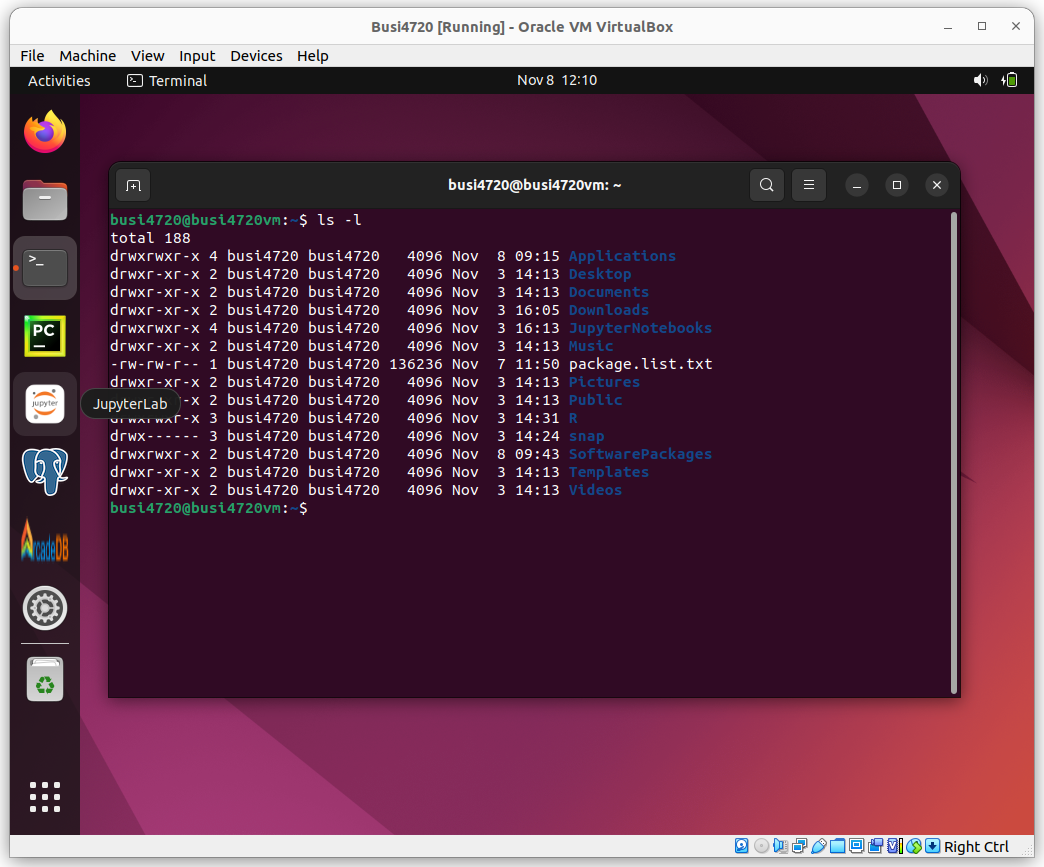
\includegraphics[height=3in]{screenshot1.png}
\end{center}

As a multi-user operating system, Ubuntu provides support for file permissions for each user, user home directories, and user privileges. User home directories are typically located in \texttt{/home/<userName>/} and the \texttt{sudo} (''\underline{s}uper\underline{u}ser do'') command may be used to execute commands as super user (equivalent to the ''root'' user in Linux terminology).
 
\begin{wrapfigure}{r}{1.in}
\begin{center}
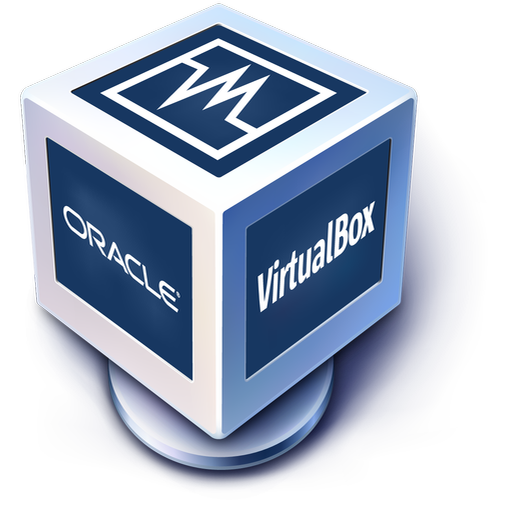
\includegraphics[height=.5in]{Virtualbox_logo.png}
\end{center}
\end{wrapfigure}
 
\section{Virtual Machines}
 
Virtualization with virtual machines allows users to create an run virtual computers on their own computers, enabling the installation and operation of multiple operating systems simultaneously. The "real" system that is running the virtualization software application is called the host system or host operating system, while the virtual computer running inside the virtualization software is called the guest system, or guest operating system. In effect, the virtualization software pretends to be an actual computer to the guest system, and the guest system is a complete operating system, such as Windows or Linux.

VirtualBox is a free and open-source virtualization software application developed by Oracle. VirtualBox is available for host systems with an Intel or AMD processor, running Windows, MacOS, or Linux operating systems. VirtualBox supports a wide range of guest operating systems, including various versions of Windows, Linux distributions, MacOS, BSD, and others. VirtualBox provides "Guest Additions," which are additional software packages that can be installed on the guest operating system. These additions enhance the performance and integration between the host and guest systems, providing features like seamless mouse integration, shared folders, and improved graphics support. 

VMWare Fusion is a proprietary virtualization software owned by Broadcom. VMWare Fusion is available for Apple Mac computers running either Intel processors (before circa 2021) or the later Apple M1, M2 or M3 processors (after circa 2021). Similar to VirtualBox, it allows users to create and run virtual machines on their computer and provides a way to share folders from the host system to the guest system, and to copy and paste from host to guest and vice versa. \\
 
\begin{tcolorbox}[colback=alert]
\noindent Virtual machine files for use with VirtualBox and VMWare Fusion are provided\footnote{\url{https://evermann.ca/busi4720.html}} that contains an Ubuntu system with all required software installed
If you wish to use this, you must install VirtualBox or VMWare Fusion on your computer, then download the corresponding virtual machine file and import it into the virtualization software application.  \\

The username is \textbf{busi4720} and the password is \textbf{busi4720}. Whenever a password is required, you should enter \textbf{busi4720}.
\end{tcolorbox}
  
\noindent \begin{tcolorbox}[colback=alert]\emph{If you do NOT wish to use the VirtualBox Appliance, you should download and install all software to your computer from the sources indicated in Table~\ref{tab:software} in (at least) the versions indicated in the table.}\end{tcolorbox}
 
\section{The Ubuntu Command Line (also for Mac Users)}

This tutorial provides a very brief introduction to the Ubuntu command line (''terminal''). The command line, also called a ''shell'' is by default the ''bash'' shell (Bourne-again shell; a pun on the earlier Bourne shell). In Ubuntu, you can open the Terminal application using the key combination \fcolorbox{black}{lightgray}{Ctrl-Alt-T}, or by selecting the Terminal application icon from the side bar or the application list. You can also open a Terminal from the file browser. \\

\noindent \emph{Note:} The default shell in the MacOS terminal is the ''zsh'' and behaves slightly differently from the bash shell. You can work with a ''bash'' shell by typing the \texttt{bash} command in a MacOS terminal.

Bash will show you a \emph{command prompt} that indicates your username (''busi4720''), the name of the computer (''busi4720vm'') and your current working directory (''$\sim$'') followed by the dollar sign ''\$''.

\noindent\underline{P}rint the \underline{w}orking \underline{d}irectory by typing the \texttt{pwd} command and then pressing the \fcolorbox{black}{lightgray}{Return} or \fcolorbox{black}{lightgray}{Enter} key:
\begin{bashcode}
busi4720@busi4720vm:~$ pwd
/home/busi4720
\end{bashcode}

\noindent\underline{M}a\underline{k}e a folder/\underline{dir}ectory with the \texttt{mkdir} command (in your current working directory):
\begin{bashcode}
busi4720@busi4720vm:~$ mkdir someFolder
\end{bashcode}
\noindent\underline{C}hange the working \underline{d}irectory to the folder you have just created with the \texttt{cd} command. Note how the Bash command prompt indicates your new working directory. 


\begin{bashcode}
busi4720@busi4720vm:~$ cd someFolder
busi4720@busi4720vm:~/someFolder$ cd ..
busi4720@busi4720vm:~$ cd ~
\end{bashcode}

\noindent The following special characters can be used when specifying folders/directories and paths:\\

\begin{tabular}{l|l} \hline
\texttt{$\sim$} & User home directory \\
\texttt{.} & Current directory \\
\texttt{..} & Upwards in the directory tree \\
\texttt{/} & Root of directory tree \\ \hline
\end{tabular} \\

\noindent Here are some tips that make working with the shell a lot easier:

\begin{itemize}
  \item Autocompletion of file names is available with the ''\fcolorbox{black}{lightgray}{Tab}'' key. When multiple file names exist that match what you have entered so far, you can enter further characters of a file name to disambiguate and press the \fcolorbox{black}{lightgray}{Tab} key again for further autocompletion. 
  \item You can recall earlier commands with the ''\fcolorbox{black}{lightgray}{Up Arrow}'' key. By default, the shell stores the last 1000 commands.
  \item You can search earlier commands with the ''\fcolorbox{black}{lightgray}{Ctrl-R}'' key. You are then prompted to search by typing in characters to find commands. The shell finds the most recent command that contains the  characters you entered. At any time you can press \fcolorbox{black}{lightgray}{Ctrl-R} again to find earlier matches to your command search. 
  \item Because the usual keys \fcolorbox{black}{lightgray}{Ctrl-X}, \fcolorbox{black}{lightgray}{Ctrl-C}, \fcolorbox{black}{lightgray}{Ctrl-V} for cutting, copying, and pasting text have different functions in the shell, you can cut, copy, and paste with the \fcolorbox{black}{lightgray}{Ctrl-Shift-X}, \fcolorbox{black}{lightgray}{Ctrl-Shift-C}, and \fcolorbox{black}{lightgray}{Ctrl-Shift-V} keys.
\end{itemize}

\noindent\underline{L}i\underline{s}t folder/directory contents using the \texttt{ls} command. The option \texttt{-l} for the command indicates that you would like to see long results. 

\scriptsize
\begin{bashcode}
busi4720@busi4720vm:~$ ls -l ~/Applications
total 8
drwxrwxr-x 7 busi4720 busi4720 4096 Nov  8 12:05 arcadedb-23.10.1
drwxr-xr-x 8 busi4720 busi4720 4096 Nov  7 11:45 pycharm-community-2
\end{bashcode}
\normalsize

\noindent The results show the total size in kB, and a list of entries:
\begin{itemize}
  \item Type of entry (''d'' = directory)
  \item Permissions for owner of the file (''rwx''), users in the same user group as the owner (''r-x'') and other users (''r-x''): \texttt{r} indicates read access, \texttt{w} indicates write access, \texttt{x} indicates permission to run the application or enter/view a directory (with \texttt{cd} or \texttt{ls}), and a \texttt{-} indicates the lack of the corresponding permission. 
  \item Names of owner and groups (''busi4720'')
  \item Size (in bytes)
  \item Last modification date and time
  \item File or directory name
\end{itemize}

\noindent Print a string of text using the \texttt{echo} command:
\begin{bashcode}
$ echo "To be or not to be"
To be or not to be
\end{bashcode}

\noindent Redirect the output of the \texttt{echo} command to a file using the \emph{redirect} symbol ''\texttt{>}''. You can redirect the output of any command this way. Use \texttt{>>} to redirect and append, instead of overwriting a file.
\small
\begin{bashcode}
$ echo "To be or not to be" > someFile.txt
$ ls -l someFile.txt
-rw-rw-r-- 1 busi4720 busi4720 19 Nov  8 14:50 someFile.txt
\end{bashcode}
\normalsize

\noindent Print contents of a file (''con\underline{cat}enate'') using the \texttt{cat} command. You can concatenate multiple files by specifying them all (this is why the command is called ''concatenate''):
\begin{bashcode}
$ cat someFile.txt
To be or not to be
\end{bashcode}

\noindent If you would like to see the contents of a file page by page or line by line, use the \texttt{less} command (a pun on ''less is more'' and the earlier ''more'' command that did the same). You will be shown the contents and can navigate up and down with the usual arrow keys.

\begin{bashcode}
$ less someFile.txt
\end{bashcode}

\noindent \underline{C}o\underline{p}y a file using the \texttt{cp} command:
\begin{bashcode}
$ cp someFile.txt someCopy.txt
\end{bashcode}

\noindent \underline{M}o\underline{v}e a file to a new location (folder/directory) using the \texttt{mv} command:
\begin{bashcode}
$ mv someCopy.txt ~/someFolder
\end{bashcode}

\noindent Renaming is moving. When you want to rename a file, move it to a new file name:
\begin{bashcode}
$ mv someFile.txt newName.txt
\end{bashcode}

\noindent \underline{R}e\underline{m}ove (delete) a file using the \texttt{rm} command:
\begin{bashcode}
$ rm someFolder/someFile.txt
\end{bashcode}

\noindent Remove a directory recursively (i.e. remove all its contents first):
\begin{bashcode}
$ rm -r ~/someFolder
\end{bashcode}

\noindent \emph{\textcolor{red}{Use this very carefully! You could inadvertently delete all your files. The shell will delete files and folders immediately and irrevocably. There is no ''undoing'' this.}} \\

\noindent View the command line \underline{history} with the \texttt{history} commands. Remember that you can redirect this output to a file if you wish or use a pipe to pipe it into the less command (see below).
\begin{bashcode}
$ history
    1  echo "To be or not to be"
    2  echo "To be or not to be" > someFile.txt
    3  ls -l someFile.txt
    4  less someFile.txt 
    5  cat someFile.txt
...
\end{bashcode}

\noindent Management of file permissions is done using the \texttt{chmod} command. You can gran and revoke read, write, and execute permissions for yourself, your group members, and other users. Remove write permission for yourself by using the \texttt{-w} option and specifying the filename:
\begin{bashcode}
$ chmod -w newName.txt
\end{bashcode}

\noindent Add write permissions using the \texttt{+w} option:
\begin{bashcode}
$ chmod +w newName.txt
\end{bashcode}

\noindent Add execute permissions using the \texttt{+x} option:
\begin{bashcode}
$ chmod +x newName.txt
\end{bashcode}

\noindent If you are stuck on how to use a command or wish to see all its options and capabilities, you can get the \underline{man}ual for a command using the \texttt{man} command:
\begin{bashcode}
$ man ls
\end{bashcode}

\noindent If you can't quite remember which command to use, you can search for commands using keywords with the \texttt{apropos} command:
\begin{samepage}
\begin{bashcode}
busi4720@busi4720vm:~$ apropos python
keyring (1)          - Python-Keyring command-line utility
pdb3 (1)             - the Python debugger
pdb3.10 (1)          - the Python debugger
pip (1)              - A tool for installing and managing Python p...
pip3 (1)             - A tool for installing and managing Python p...
py3compile (1)       - byte compile Python 3 source files
py3versions (1)      - print python3 version information
pydoc3 (1)           - the Python documentation tool
pydoc3.10 (1)        - the Python documentation tool
pygettext3 (1)       - Python equivalent of xgettext(1)
pygettext3.10 (1)    - Python equivalent of xgettext(1)
python (1)           - an interpreted, interactive, object-oriente...
python3.10-config (1) - output build options for python C/C++ exte...
python3 (1)          - an interpreted, interactive, object-oriente...
...
\end{bashcode}
\end{samepage}

\noindent You can see a list of all processes currently running using the \texttt{ps} command. The results show the process identifier (PID), the console from which you started the process, the computing time it has consumed, and the command that was used to start the process. Add the \texttt{a} and \texttt{x} option to see \emph{all} the processes running on your computer, not just the processes you have started.
\begin{bashcode}
$ ps ax
    PID TTY          TIME CMD
   3024 pts/0    00:00:00 bash
   3151 pts/0    00:00:00 ps
\end{bashcode}

\noindent The \texttt{grep} command is useful to find something in a file or input stream. Use it as in the following example in a pipe:
\begin{bashcode}
$ cat newName.txt | grep be
$ ls -l | grep .txt
$ history | grep .txt
\end{bashcode}

\noindent \emph{Note:} The vertical bar is called a \emph{''pipe''}, it pipes the output of one command as input into the next one

\noindent The following are further beginner-level tutorials on using the command line on Ubuntu (or really any Linux distribution):
\begin{itemize}
\item \href{https://ubuntu.com/tutorials/command-line-for-beginners}{Ubuntu command line for beginners}
\item \href{https://www.digitalocean.com/community/tutorials/a-linux-command-line-primer}{Linux command line primer}
\item \href{https://www.digitalocean.com/community/tutorial-series/getting-started-with-linux}{Getting started with Linux}
\end{itemize}

\section{Review Questions}

\paragraph*{General}
\begin{enumerate}[nosep]
	\item What is the definition of ''data analytics''? What is "business analytics"?
	\item What is the relationship between data management and analytics?
	\item Give examples of areas related to analytics and their relationships.
	\item Why is text analysis mentioned in connection with machine learning?
	\item What are artificial neural networks (ANN) and deep neural networks (DNN), and how are they the same and how are they different from linear regression models?
	\item In what way does AI include areas beyond machine learning?
	\item Characterize Big Data and its focus.
	\item Provide an example that illustrates areas of AI outside of data analytics.
	\item Define techniques in the context of data science.
    \item Provide an example of a technique used in exploratory data analysis.
	\item Mention a few examples of tools used in data science.
	\item Explain the relationship between methods and techniques in data science.
	\item Provide examples of tasks or challenges that high-level methodologies (methods) might address in data science.
	\item Summarize the roles of methods, techniques, and tools in the context of data science.
\end{enumerate}
\paragraph*{Types of Analytics}
\begin{enumerate}[nosep,resume*]
	\item What is the primary purpose of descriptive analytics? Give an example of how it might be used in a business context?
	\item Explain how predictive analytics differs from descriptive analytics. Illustrate with an example how a simple linear regression model can be used in predictive analytics.
    \item Describe prescriptive analytics and how it differs from predictive analytics. 
    \item What is visual analytics and how does it support human tasks in data analysis? Discuss how it can contribute to other types of analytics.
    \item Compare and contrast predictive and prescriptive analytics in terms of their approach and end goals. How do they both utilize past data?
    \item If a company wants to understand its sales performance over the last five years, which type of analytics would be most appropriate and why?
    \item Imagine a scenario where a company needs to decide on future marketing strategies. Which type of analytics would be most beneficial for them and how might it be implemented?
\end{enumerate}
\paragraph*{Learning}
\begin{enumerate}[nosep,resume*]
	\item What is supervised learning in machine learning, and how does it differ from unsupervised learning?
	\item Describe how a simple linear regression model works in supervised learning. What are the key parameters in this model?
    \item Compare the simplicity of a linear regression model with the complexity of a model like GPT in supervised learning. What are the key differences?
    \item Provide examples of tasks that are typically performed using unsupervised learning.
	\item How is clustering used in unsupervised learning, and can you give an example of its application in a business context?
	\item Explain the concept of dimensionality reduction in unsupervised learning and its potential benefits.
\end{enumerate}

\section{Hands-On Exercises}

The following are a set of connected exercises to help you practice your command line skills. Do them in the order listed.

\begin{enumerate}
\item Navigation and Listing
\begin{enumerate}[nosep]
	\item Open the terminal and use the \texttt{pwd} command to print the current working directory.
	\item Use \texttt{ls} to list the contents of the current directory.
	\item Create a new directory named "Exercise1" using \texttt{mkdir}.
	\item Navigate into the "Exercise1" directory using \texttt{cd}.
\end{enumerate}
\item File Manipulation
\begin{enumerate}[nosep,resume*]
	\item Create a new file named "file1.txt" inside the "Exercise1" directory using \texttt{touch}.
	\item Use \texttt{cat} to display the contents of "file1.txt".
	\item Append the text "Hello, Bash!" to "file1.txt" using \texttt{echo} and \texttt{>>}.
	\item Display the updated contents of "file1.txt" using \texttt{cat}.
\end{enumerate}
\item Removing and Renaming
\begin{enumerate}[nosep,resume*]
	\item Remove "file1.txt" using the \texttt{rm} command.
	\item Create a copy of the "Exercise1" directory named "Exercise1\_backup" using \texttt{cp -r}.
	\item Remove the original "Exercise1" directory using \texttt{rm -r}.
\end{enumerate}
\item Directory Manipulation
\begin{enumerate}[nosep,resume*]
	\item Recreate the "Exercise1" directory.
	\item Create three subdirectories inside "Exercise1" named "Subdir1", "Subdir2", and "Subdir3" using \texttt{mkdir}.
	\item List the contents of "Exercise1" to verify the creation of subdirectories.
\end{enumerate}
\item Searching and Filtering
\begin{enumerate}[nosep,resume*]
	\item Create a file named "keywords.txt" inside "Exercise1" and add some random text.
	\item Use \texttt{grep} to search for a specific word (e.g., "Bash") in "keywords.txt".
	\item Create a new file named "filtered.txt" and use \texttt{grep} to filter lines containing the word you searched for in "keywords.txt".
\end{enumerate}
\item Process Management
\begin{enumerate}[nosep,resume*]
	\item Use \texttt{ps} to display information about the current processes running on your system.
	\item Use \texttt{ps aux | grep bash} to filter and display information about Bash processes.
\end{enumerate}
\item Cleanup
\begin{enumerate}[nosep,resume*]
	\item Remove the entire "Exercise1" directory and its contents using \texttt{rm -r}.
	\item Confirm that the "Exercise1" directory no longer exists by listing the contents of the current directory.
\end{enumerate}
\end{enumerate}

